\chapter{Large language models}



\section{Decoder-only architecture} \label{sec:llm}

\begin{description}
    \item[Conditional generation] \marginnote{Conditional generation}
        Generate text conditioned on the input tokens (i.e., prompt).

        \begin{figure}[H]
            \centering
            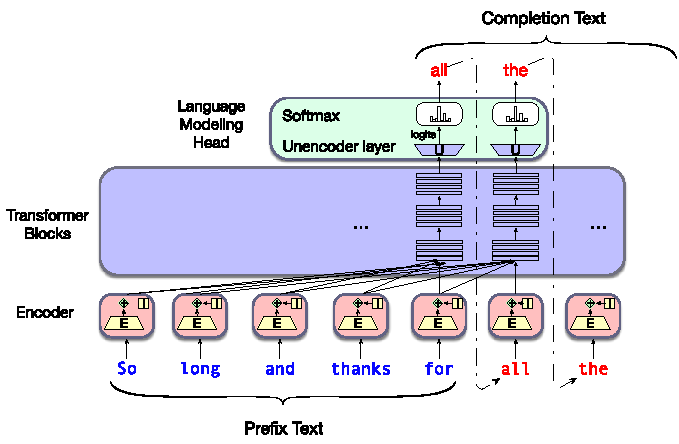
\includegraphics[width=0.45\linewidth]{./img/_conditional_generation.pdf}
        \end{figure}

        \begin{example}[Sentiment analysis]
            Given the prompt:
            \[ p = \texttt{the sentiment of the sentence `I like Jackie Chan' is} \]
            Determine the probability of the tokens \texttt{positive} and \texttt{negative}:
            \[
                \prob{\texttt{positive} \mid p} \qquad \prob{\texttt{negative} \mid p}
            \]
        \end{example}

        \begin{example}[Question answering]
            Given the prompt:
            \[ p = \texttt{Q: who wrote the book `The origin of Species'? A:} \]
            Determine the tokens of the answer autoregressively:
            \[
                \arg\max_{w_1} \prob{w_1 \mid p}, \arg\max_{w_2} \prob{w_2 \mid pw_1}, \dots
            \]
        \end{example}
\end{description}


\subsection{Decoding strategies}

\begin{description}
    \item[Greedy decoding] \marginnote{Greedy decoding}
        Select the next token as the most probable of the output distribution.

        \begin{remark}
            Greedy decoding risks getting stuck in a local optimum.

            \indenttbox
            \begin{example}
                Consider the following search tree of possible generated sequences:

                \begin{minipage}{0.35\linewidth}
                    \begin{figure}[H]
                        \centering
                        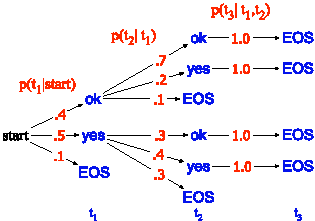
\includegraphics[width=\linewidth]{./img/_greedy_decoding_local_minimum.pdf}
                    \end{figure}
                \end{minipage}
                \hfill
                \begin{minipage}[b]{0.6\linewidth}
                    Greedy search would select the sequence \texttt{yes yes} which has probability $0.5 \cdot 0.4 = 0.2$. However, the sequence \texttt{ok ok} has a higher probability of $0.4 \cdot 0.7 = 0.28$.
                \end{minipage}
            \end{example}
        \end{remark}

    \item[Beam search] \marginnote{Beam search}
        Given a beam width $k$, perform a breadth-first search keeping at each branching level the top-$k$ tokens based on the probability of that sequence:
        \[ \log\left( \prob{y \mid x} \right) = \sum_{i=1}^{t} \log\left( \prob{ y_i \mid x, y_1, \dots, y_{i-1} } \right) \]

        \begin{example}
            Consider the following tree with beam width $k=2$:
            \begin{figure}[H]
                \centering
                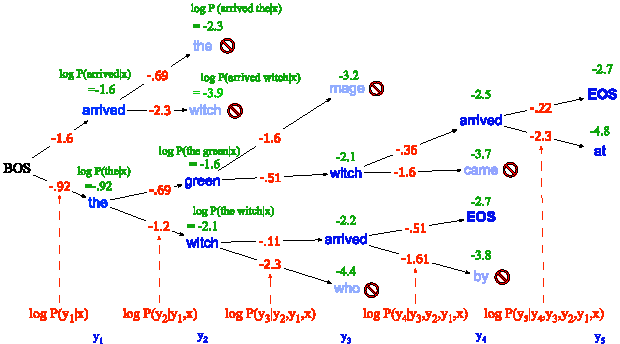
\includegraphics[width=0.7\linewidth]{./img/_beam_search.pdf}
            \end{figure}
            The selected sequence is \texttt{[BOS] the green witch arrived [EOS]}.
        \end{example}

        \begin{remark}
            As each path might generate sequences of different length, the score is usually normalized by the number of tokens as:
            \[ \log\left( \prob{y \mid x} \right) = \frac{1}{t} \sum_{i=1}^{t} \log\left( \prob{ y_i \mid x, y_1, \dots, y_{i-1} } \right) \]
        \end{remark}

        \begin{remark}
            The likelihood of the sequences generated using beam search is higher than using greedy decoding. However, beam search is still not optimal.
        \end{remark}

    \item[Sampling] \marginnote{Sampling}
        Sample the next token based on the output distribution.

        \begin{description}
            \item[Random sampling]
                Sample considering the distribution over the whole vocabulary.

                \begin{remark}
                    By adding-up all the low-probability words (which are most likely unreasonable as the next token), their actual chance of getting selected is relatively high.
                \end{remark}

            \item[Temperature sampling]
                Skew the distribution to emphasize the most likely words and decrease the probability of less likely words. Given the logits $\vec{u}$ and the temperature $\tau$, the output distribution $\vec{y}$ is determined as:
                \[ \vec{y} = \texttt{softmax}\left( \frac{\vec{u}}{\tau} \right) \]
                where:
                \begin{itemize}
                    \item Higher temperatures (i.e., $\tau > 1$) allow for considering low-probability words.
                    \item Lower temperatures (i.e., $\tau \in (0, 1]$) focus on high-probability words.
                    \begin{remark}
                        A temperature of $\tau = 0$ corresponds to greedy decoding.
                    \end{remark}
                \end{itemize}


            \item[Top-k sampling]
                Consider the top-$k$ most probable words and apply random sampling on their normalized distribution.

                \begin{remark}
                    $k=1$ corresponds to greedy decoding.
                \end{remark}

                \begin{remark}
                    $k$ is fixed and does not account for the shape of the distribution.
                \end{remark}

            \item[Top-p/nucleus sampling]
                Consider the most likely words such that their probability mass adds up to $p$. Then, apply random sampling on their normalized distribution.
        \end{description}
\end{description}


\subsection{Pre-training}

\begin{description}
    \item[Pre-training] \marginnote{Pre-training}
        Use self-supervision and teacher forcing to train the whole context window in parallel on a large text corpus.

        \begin{remark}
            Results are highly dependent on the training corpora. Important aspects to consider are:
            \begin{descriptionlist}
                \item[Language] Most of the available data is in English.
                \item[Data quality] Prefer high-quality sources such as Wikipedia or books. Boilerplate removal and deduplication might be needed. 
                \item[Safety filtering] Toxicity removal might be needed
                \item[Ethical and legal issues] Use of copyrighted material, permission from data owners, use of private information, \dots
            \end{descriptionlist}
        \end{remark}

    \item[Scaling laws] \marginnote{Scaling laws}
        Empirical laws that put in relationship:
        \begin{itemize}
            \item Non-embedding parameters $N$ ($N \approx 2 d_\text{model} n_\text{layer} (2 d_\text{attention} + d_\text{ff})$),
            \item Training data size $D$,
            \item Compute budget $C$ (i.e., training iterations).
        \end{itemize}
        By keeping two of the three factors constant, the loss $\mathcal{L}$ of an LLM can be estimated as a function of the third variable:
        \[ 
            \mathcal{L}(N) = \left( \frac{N_c}{N} \right)^{\alpha_N} 
            \qquad
            \mathcal{L}(D) = \left( \frac{D_c}{D} \right)^{\alpha_D} 
            \qquad
            \mathcal{L}(C) = \left( \frac{C_c}{C} \right)^{\alpha_C} 
        \]
        where $N_c$, $D_c$, $C_c$, $\alpha_N$, $\alpha_D$, and $\alpha_C$ are constants determined empirically based on the model architecture.
\end{description}


\subsection{Fine-tuning}

\begin{description}
    \item[Fine-tuning] \marginnote{Fine-tuning}
        Specialize an LLM to a specific domain or task.

        \begin{description}
            \item[Continued pre-training] \marginnote{Continued pre-training}
                Continue pre-training with a domain-specific corpus.

            \item[Model adaptation]
                Specialize a model by adding new learnable parameters.

                \begin{description}
                    \item[Parameter-efficient fine-tuning (PEFT)] \marginnote{Parameter-efficient fine-tuning (PEFT)}
                        Continue training a selected subset of parameters (e.g., LoRA \Cref{sec:lora}).

                    \item[Task-specific fine-tuning] \marginnote{Task-specific fine-tuning}
                        Add a new trainable head on top of the model.
                \end{description}

            \item[Supervised fine-tuning] \marginnote{Supervised fine-tuning}
                Continue training using a supervised dataset to align the model to human's expectation.
        \end{description}
\end{description}



\section{Encoder-only architecture} \label{sec:mlm}

\begin{description}
    \item[Transformer encoder] \marginnote{Transformer encoder}
        Architecture that produces contextual embeddings by considering both left-to-right and right-to-left context.

        \begin{remark}
            This architecture does feature extraction and is more suited for classification tasks.
        \end{remark}

        \begin{description}
            \item[Architecture]
                Similar to a transformer decoder, but self-attention is not causal.

                \begin{figure}[H]
                    \centering
                    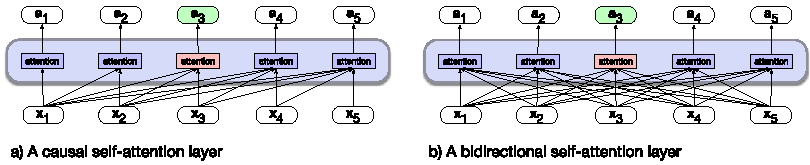
\includegraphics[width=0.75\linewidth]{./img/_decoder_vs_encoder.pdf}
                \end{figure}
        \end{description}

    \item[Contextual embedding] \marginnote{Contextual embedding}
        Represent the meaning of word instances (i.e., dynamically depending on the surroundings).

        \begin{remark}[Sequence embedding]
            Encoders usually have a classifier token (e.g., \texttt{[CLS]}) to model the whole sentence.
        \end{remark}

        \begin{example}[Word sense disambiguation]
            Task of determining the sense of each word of a sequence. Senses usually come from an existing ontology (e.g., WordNet). An approach to solve the problem is the following:
            \begin{enumerate}
                \item Compute the embedding $\vec{v}_i$ of words using a pre-trained encoder (e.g., BERT).
                \item Represent the embedding of a sense as the average of the tokens of that sense:
                \[ \vec{v}_s = \frac{1}{n} \sum_i \vec{v}_i \]
                \item Predict the sense of a word $\vec{t}$ as:
                \[ \arg\max_{s \in \texttt{senses}(\vec{t})} \texttt{distance}(\vec{t}, \vec{v}_s) \]
            \end{enumerate}
        \end{example}
\end{description}

\begin{description}
    \item[Tokenizer fertility] \marginnote{Tokenizer fertility}
        Average amount of tokens used to represent words.

        \begin{remark}
            Tokenizer fertility is relevant for inference speed.
        \end{remark}

    \item[Curse of multilinguality] \marginnote{Curse of multilinguality}
        The performance of each language of a multilingual model tend to be worse than its monolingual counterpart.
\end{description}


\subsection{Pre-training}

\begin{description}
    \item[Masked language modelling] \marginnote{Masked language modelling}
        Task of predicting missing or corrupted tokens in a sequence.

        \begin{remark}
            Transformer encoders output embeddings. For training purposes, a head to output a distribution over the vocabulary is added.
        \end{remark}

        \begin{example}
            Given a training corpus, BERT is trained by randomly sampling $15\%$ of the tokens in the training data and either:
            \begin{itemize}
                \item Mask it with a special \texttt{[MASK]} token ($80\%$ of the time).
                \item Replace it with a different token ($10\%$ of the time).
                \item Do nothing ($10\%$ of the time).
            \end{itemize}

            \begin{figure}[H]
                \centering
                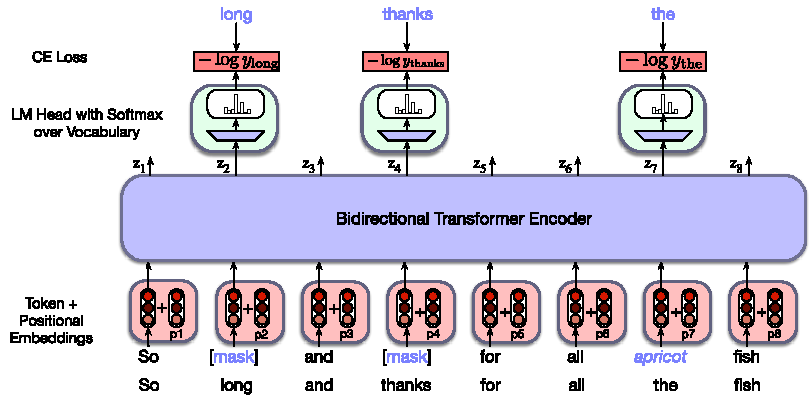
\includegraphics[width=0.6\linewidth]{./img/_bert_training.pdf}
            \end{figure}

            \indenttbox
            \begin{remark}
                BERT's training approach is inefficient as masks are determined before training and only $15\%$ of the corpus tokens are actually used for training. Other models (e.g., RoBERTa), dynamically determine the mask at training time, allowing for more variety.
            \end{remark}
        \end{example}

    \item[Span masking] \marginnote{Span masking}
        Mask contiguous spans of words to obtain a harder training objective.

        \begin{remark}
            This approach generally produces better embeddings.
        \end{remark}
\end{description}


\subsection{Fine-tuning}

\begin{description}
    \item[Fine-tuning for classification]
        Add a classification head on top of the classifier token.

    \item[Fine-tuning for sequence-pair classification]
        Use a model pre-trained to process pair of sequences. This is usually done by means of a special separator token (e.g., \texttt{[SEP]} in BERT).

    \item[Fine-tuning for sequence labeling]
        Add a classification head on top of each token. A conditional random field (CRF) layers can also be added to produce globally more coherent tags.

        \begin{description}
            \item[Named entity recognition (NER)] \marginnote{Named entity recognition (NER)}
            Task of assigning to each word of a sequence its entity class. NER taggers usually also capture concepts spanning across multiple tokens. To achieve this, additional information is provided with the entity class:
            \begin{descriptionlist}
                \item[Begin] Starting token of a concept.
                \item[Inside] Token belonging to the same span of the previous one.
                \item[End] Last token of a span.
                \item[Outside] Token outside the scope of the tagger.
            \end{descriptionlist}

            \begin{description}
                \item[Metrics] \phantom{}
                    \begin{description}
                        \item[Recall] $\frac{\text{Correctly labeled responses}}{\text{Total that should have been labeled}}$
                        \item[Precision] $\frac{\text{Correctly labeled responses}}{\text{Total that has been labeled}}$
                    \end{description}

                    \begin{remark}
                        The entity (so, also a span of text) is the atomic unit for NER metrics.
                    \end{remark}
            \end{description}
        \end{description}
\end{description}


\begin{remark}[GLUE]
    The General Language Understanding Evaluation (GLUE) benchmark is a common set of tasks used to evaluate natural language understanding models. It comprises tasks based on single sentences, multiple sentences, and inference from a sequence.
\end{remark}



\section{Encoder-decoder architecture}

\begin{description}
    \item[Encoder-decoder architecture] \marginnote{Encoder-decoder architecture}
        Model with both an encoder and decoder:
        \begin{descriptionlist}
            \item[Encoder] 
                Architecture as presented in \Cref{sec:mlm}. Its result is used to condition the output of the decoder.
            \item[Decoder] 
                Architecture similar to the one presented in \Cref{sec:llm} with an additional cross-attention layer inserted before causal attention.

                \begin{description}
                    \item[Cross-attention] \marginnote{Cross-attention}
                        Attention layer that uses the output of the encoder as keys and values, while the query is from the decoder.
                \end{description}
        \end{descriptionlist}

        \begin{figure}[H]
            \centering
            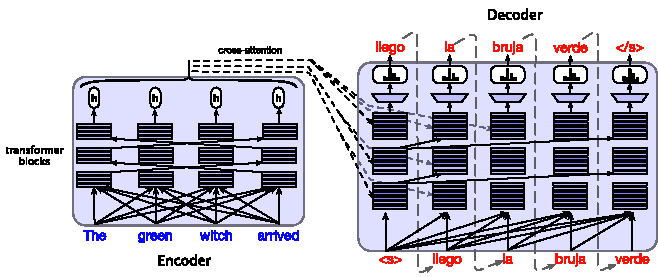
\includegraphics[width=0.7\linewidth]{./img/_encoder_decoder.pdf}
        \end{figure}
\end{description}


\subsection{Pre-training}

\begin{description}
    \item[Span corruption] \marginnote{Span corruption}
        Given an input sequence, replace different-length spans of text with a unique placeholder. The encoder takes as input the corrupted sequence, while the decoder has to predict the missing words.

        \begin{remark}
            It has been observed that targeted span masking works better compared to random span masking.
        \end{remark}

        \begin{example}
            Given the sequence:
            \[ \texttt{<bos> thank you \underline{for inviting} me to your party \underline{last} week <eos>} \]
            Some spans of text are masked with placeholder tokens as follows:
            \[ \texttt{<bos> thank you <X> me to your party <Y> week <eos>} \]
            The masked sequence is passed through the encoder, while the decoder has to predict the masked tokens:
            \[ \texttt{<bos> <X> for inviting <Y> last <Z> <eos>} \]
        \end{example}
\end{description}